\documentclass{Base}
\usepackage{framed}
\usepackage[outerbars]{changebar}

\usepackage{amsmath}    % assumes amsmath package installed
\usepackage{amssymb}    % assumes amsmath package installed
\usepackage{mathtools}  % assumes amsmath package installed                            
%
\usepackage{makeidx}         % allows index generation
\usepackage{graphicx}        % standard LaTeX graphics tool
                             % when including figure files
\usepackage{multicol}        % used for the two-column index
\usepackage{booktabs,tabularx}
\usepackage{multirow}

\usepackage[a4paper]{geometry}
\geometry{left=4.5cm}
\geometry{right=4.5cm}

\usepackage{accents}
\newcommand{\ubar}[1]{\underaccent{\bar}{#1}}

\usepackage{enumitem}
\newcommand{\subscript}[2]{$#1 _ #2$}

\usepackage[ruled,vlined]{algorithm2e}

\usepackage[capitalize]{cleveref}

\begin{document}
\clearpage
%% temporary titles
% command to provide stretchy vertical space in proportion
\newcommand\nbvspace[1][3]{\vspace*{\stretch{#1}}}
% allow some slack to avoid under/overfull boxes
\newcommand\nbstretchyspace{\spaceskip0.5em plus 0.25em minus 0.25em}
% To improve spacing on titlepages
\newcommand{\nbtitlestretch}{\spaceskip0.6em}
\pagestyle{empty}
\begin{center}
\centering % Centre everything on the title page
	
	\scshape % Use small caps for all text on the title page
	
	\vspace*{\baselineskip} % White space at the top of the page
	
	%------------------------------------------------
	%	Title
	%------------------------------------------------
	
	\rule{\textwidth}{1.6pt}\vspace*{-\baselineskip}\vspace*{2pt} % Thick horizontal rule
	\rule{\textwidth}{0.4pt} % Thin horizontal rule
	
	\vspace{0.75\baselineskip} % Whitespace above the title
	
	{\LARGE NOTES ON MIXED-INITIATIVE CONTROL\\} % Title
	
	\vspace{0.75\baselineskip} % Whitespace below the title
	
	\rule{\textwidth}{0.4pt}\vspace*{-\baselineskip}\vspace{3.2pt} % Thin horizontal rule
	\rule{\textwidth}{1.6pt} % Thick horizontal rule
	
	\vspace{2\baselineskip} % Whitespace after the title block
	
	%------------------------------------------------
	%	Subtitle
	%------------------------------------------------
	
	An optimization-based approach % Subtitle or further description
	
	\vspace*{3\baselineskip} % Whitespace under the subtitle
	
	%------------------------------------------------
	%	Editor(s)
	%------------------------------------------------
	
	Written By
	
	\vspace{0.5\baselineskip} % Whitespace before the editors
	
	{\scshape\Large B\'arbara Barros Carlos \\} % Editor list
	
	\vspace{0.5\baselineskip} % Whitespace below the editor list
	
	\textit{DIAG Robotics Lab \\ Sapienza Universit\`a di Roma} % Editor affiliation
	
	\vfill % Whitespace between editor names and publisher logo
	
	%------------------------------------------------
	%	Publisher
	%------------------------------------------------
	
	
	\vspace{0.3\baselineskip} 
	
	July, 2020 % Publication year
	
\end{center}

\chapter{Adaptive Zone NMPC with Trajectory-Dependent Penalties for Mixed-Initiative Control}

%  SECTIONS   %
%%%%%%%%%%%%%%%%%%%%%%%%%%%%%%%%%%%%%%%%%%%%%%%%%%%%%%%%%%%%%%%%%%%%%%%%%%%%%%%%%%%%%%
\section{Main Idea}
I try to explain in simple words without formulas the main idea of the framework. the nomenclature is completely tentative.

%%% ---------------------------------------------------------------
\subsection{Problem setting}
%%% ---------------------------------------------------------------

\subsubsection{Robot} The robot is represented by a certain dynamical system and a set of `dynamical constraints' on the system variables.


\subsubsection{Working conditions}
Certain given conditions are given and represent the minimum requirements that the robot has to obey to operate `healthy', let us call them the `working conditions'. These can contain both safety rules (e.g., maximum kinetic energy, minimum distances from obstacles etc.) and/or task related rules (e.g., accuracy of end-effector positioning, orientation, etc.)

\subsubsection{Fully autonomous controller and cost} 
An automatic receding horizon controller is given that is able to ensure that the robot satisfies both dynamical constraints and the working conditions. We call this the `fully-autonomous controller' and the corresponding cost function is called the `fully-autonomous cost'.

\subsubsection{Human inputs}
The human is given the possibility to specify desired values for some of the system variables, either directly for some of the variable or in an implicit way (specifying the desired value of a function of the variables), these are called `human inputs'.

\subsubsection{Objective} 
Let the robot obey as much as possible to the human inputs while maintaining the working conditions and the dynamical constraints.


%%% ---------------------------------------------------------------
\subsection{Our proposed solution}
%%% ---------------------------------------------------------------

The objective is twofold, from one side we want the human input to be obeyed as much as possible and from the other side we want to keep valid the working conditions and dynamical constraints all the time. We know that the latter objective would be fulfilled if we  let the robot be always controlled by the fully-autonomous controller. However this alone would not ensure the first objective.


\subsubsection{Predicted healthiness index} 

At each time instant we simulate what would be the system behavior starting from the current measured state under the effect of the fully autonomous controller within the controller time horizon. From the simulated behavior we compute how far the robot is from violating the working conditions within the horizon. A certain continuous function between 0 and 1, named the `predicted healthiness index', is then computed in a way that its value is 0 if the violation is too close and 1 if it is far enough. The idea is that the closer the index to 0 the more troublesome will be to keep the system within the working condition in the next horizon, even if full control is given to the fully autonomous controller (and human inputs are completely disregarded that moment on). Viceversa, the closer the index to 1 the easier the job of the fully autonomous controller will be in case it takes full control of the system.

\subsubsection{Actual robot controller} 

We let the robot be controlled by a receding horizon controller which is a copy of the full autonomous controller a part from a major difference, its cost function, named the `actual robot cost', is a convex combination between the fully autonomous cost and the `human input cost'. The latter is a cost term which penalizes the divergence from the human inputs. The convex combination is driven by the  Predicted healthiness index, when the index tends to 0 the actual robot cost tends to the fully-autonomous cost, when the index tends to 1 the actual robot cost tends to the human input cost.





%%%%%%%%%%%%%%%%%%%%%%%%%%%%%%%%%%%%%%%%%%%%%%%%%%%%%%%%%%%%%%%%%%%%%%%%%%%%%%%%%%%%%%
\section{Introduction}
This chapter presents a novel zone \textcolor{red}{AF: is this 'zone' a term used in the literature or is a novel term?} nonlinear model predictive control (NMPC) for mixed-inititiative control. A zone NMPC relies on a dynamic cost function that updates its state and control penalty parameters in real-time according to predicted trajectories. The criteria for adapting the parameters are based on zone-excursion functions that determine \textcolor{blue}{how the control authority between the human and the robot must be mixed at each sampling instant}. 

The proposed mixed-initiative control algorithm is evaluated considering a semi-autonomous task, in which a quadrotor must be steered by a human operator through a pre-established navigation plan. Three different levels of piloting skill in humans are regarded, ranging from inexperienced to highly experienced. The results indicate that the approach operates efficiently and safely, even in scenarios of weak piloting skills, reducing the risks of crashes. 
%%%%%%%%%%%%%%%%%%%%%%%%%%%%%%%%%%%%%%%%%%%%%%%%%%%%%%%%%%%%%%%%%%%%%%%%%%%%%%%%%%%%%%
\section{Problem Formulation}
\textcolor{red}{AF: one thing is the problem and a different one is the solution, this section seems to talk about the solution, not the problem. A section about the problem should be added,}

\textcolor{red}{AF: a block diagram must be added and referred to.}

\begin{figure*}
	\centering
	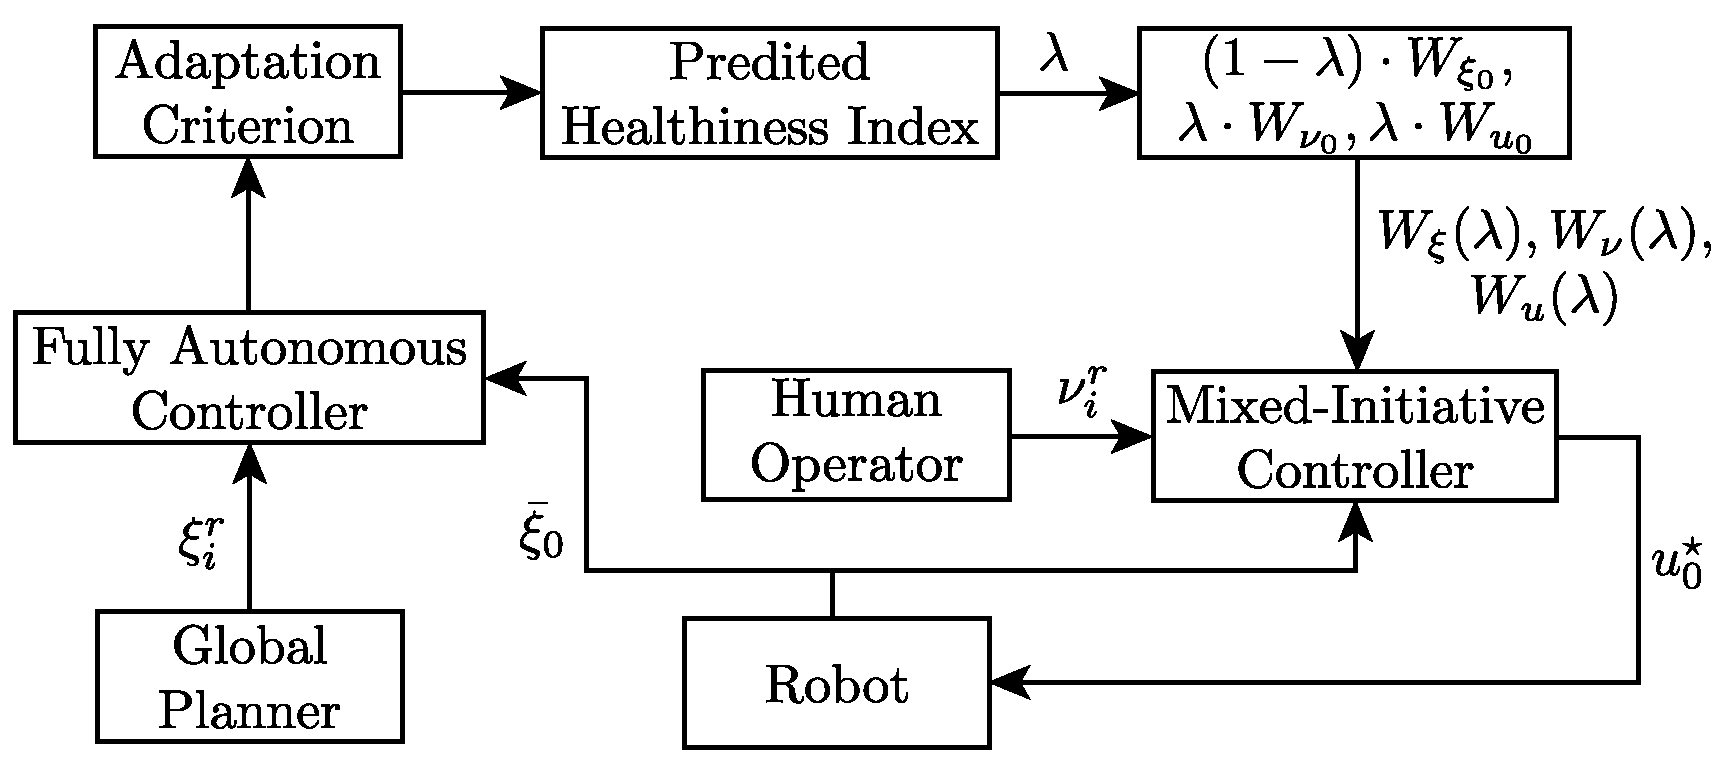
\includegraphics[width=1.0\textwidth]{figure/block_diagram}
\end{figure*}

The base controller of this work is a zone NMPC with trajectory-dependent penalty parameters. The zone NMPC model takes into account the robot dynamics plus part of the robot dynamics that the human is able to control, e.g. attitude and height \textcolor{red}{AF: to be checked}). The controller is driven by the predicted trajectories from another NMPC (namely, low-level NMPC), which considers just the dynamics of the robot. At each time instant, two constrained optimization problems are solved numerically, yielding two different feedback control policies.

In this section, we present the respective prediction models for each NMPC, as well as the nonlinear programs (NLP) arising in each NMPC formulation. 
%%%%%%%%%%%%%%%%%%%%%%%%%%%%%%%%%%%%%%%%%%%%%%%%%%%%%%%%%%%%%%%%%%%%%%%%%%%%%%%%%%%%%%
\subsection{Prediction Models}
Let $\{\mathcal{B}\}$ be the body-fixed frame, located at the center of mass (CoM) of a quadrotor, aligned with the North-West-Up (NWU) inertial frame $\{\mathcal{I}\}$. In order to implement the low-level NMPC, we consider a nonlinear dynamic model of the form
\begin{equation*}
	\dot{\xi} = f_1(\xi,u).
\end{equation*}
We then define the state vector, considering only the dynamics of the robot:
\begin{equation*}
	\xi := (p,\gamma,v_b,\omega,\Omega)^T \in \mathbb{R}^{16},
\end{equation*}
where $ p := (x, y, z)$  is the position vector in $\{\mathcal{I}\}$, $ \gamma := (\phi,\theta,\psi)$ are the Euler angles for orientation, $v_b := (v_x, v_y, v_z)$ is the linear velocities vector in $\{\mathcal{B}\}$, $\omega := (\omega_x, \omega_y, \omega_z)$ is the vector of angular rates, and finally $\Omega := (\Omega_1,\Omega_2,\Omega_3,\Omega_4)$ is the vector containing the rotation speed of the propellers. Hence, we regard the following quadrotor model:
 \begin{equation*}
 	\begin{aligned}
 	\dot{p} &= Rv_b \\
 	\dot{\gamma} &= T \omega\\
	\dot{v}_b &= \frac{1}{m}F - R^{T}G - \omega\times v_b\\
	\dot{\omega} &= J^{-1}(M - \omega\times J\omega)\\
	\dot{\Omega} &= \frac{\tau}{J_m},
 	\end{aligned}%
 \end{equation*}
 \textcolor{red}{AF: what about drag of the rotor in the motor equation?}
where the mass of the quadrotor is $m \in \mathbb{R}^+$, and $G \vcentcolon =(0, 0, mg)^T$ with $g$ being the gravitational acceleration. The robot inertia matrix with respect to its CoM and expressed in $\{\mathcal{B}\}$ is given by $J \vcentcolon = \text{diag}(J_{xx}, J_{yy}, J_{zz}) \in \mathbb{R}^{3 \times 3}$. The rotation matrix from  $\{\mathcal{B}\}$ to $\{\mathcal{I}\}$ is expressed as $R \in SO(3)$. The matrix $T \vcentcolon \mathbb{R}^3 \rightarrow \mathbb{R}^{3 \times 3}$ represents the relation between the instantaneous rates of change of the Euler angles and the instantaneous components of $\omega$. \textcolor{red}{AF: define ALL the symbols introduced, here and after} The total external forces and moments applied to the CoM of quadrotor in $\{\mathcal{B}\}$ are defined as 
 \begin{equation}
 	\begin{aligned}
    F & \vcentcolon =  \sum_{i=1}^4 C_T\Omega_{i}^2\mathbf{1}_z, \quad M \vcentcolon = (M_x, M_y, M_z)^T
	\end{aligned}
 \end{equation}\label{eq:force_moments}
 with
 \begin{equation*}
 	\begin{aligned}
    M_x &= C_T\cdot l(-\Omega_{1}^{2}-\Omega_{2}^{2}+\Omega_{3}^{2}+\Omega_{4}^{2}),\\
    M_y &= C_T\cdot l(-\Omega_{1}^{2}+\Omega_{2}^{2}+\Omega_{3}^{2}-\Omega_{4}^{2}),\\
    M_z &= C_D(-\Omega_{1}^{2}+\Omega_{2}^{2}-\Omega_{3}^{2}+\Omega_{4}^{2}),
 	\end{aligned}
 \end{equation*}
where $C_T$ is the thrust coefficient, $C_D$ is the drag coefficient, and $l$ is half of the distance between motors. When considering a medium-size quadrotor, the rotor inertia $J_m$ is not negligible as the radius of the rotor's axle is not small. Therefore, we consider the rotor torques as the control inputs of this system
\begin{equation}
	u := (\tau_1,\tau_2,\tau_3,\tau_4)^T \in \mathbb{R}^4.\label{eq:control_inputs}
\end{equation}



Moreover, for the zone NMPC let us consider the following nonlinear dynamic model:
\begin{equation*}
	\dot{\sigma} = f_2(\sigma,u).
\end{equation*}
This model is composed of the robot dynamics plus part of the robot dynamics that the human is able to control. For a quadrotor, the latter is essentially composed of the rotational dynamics and the translational dynamics in $z$ (which is directly linked to the collective speed of the propellers). Thus, we can formally define the part of the dynamics controlled by the human as:
\begin{equation*}
	\nu \vcentcolon = (\gamma, \omega, \Omega)^T \in \mathbb{R}^{10}.
\end{equation*}
Then, the state vector of the zone NMPC can be characterized as follows:
\begin{equation*}
	\sigma \vcentcolon = (p,\gamma,v_b,\omega,\Omega,\nu)^T \in \mathbb{R}^{26},
\end{equation*}
while the control inputs are the rotor torques, likewise regarded in \eqref{eq:control_inputs}.



\textcolor{red}{AF: this is confusing. Some of the states seem to appear twice. I would rather say that in this controller there are some additional exogenous inputs provided by the human which are the desired orientation and desired total thrust and give to these quantities a different name. In any case these quantities should not appear in the state of the robot, in the sense that they do not affect the robot dynamics directly, but rather in the objective function, i.e., in the controlled (closed loop) dynamics, in the same way the desired trajectory appear.}


%%%%%%%%%%%%%%%%%%%%%%%%%%%%%%%%%%%%%%%%%%%%%%%%%%%%%%%%%%%%%%%%%%%%%%%%%%%%%%%%%%%%%%
\subsection{Nonlinear Programs}
When using NMPC to control a system, at each sampling instant, a nonlinear nonconvex program is solved using the current state as the initial value. However, as the programs' solution times can be rather long, the employment of NMPC has only recently been extended to applications where shorter sampling times are required \cite{barros2020b}. Typically, a continuous-time, infinite-dimensional optimal control problem (OCP) is tailored according to the problem at hand, discretized using some numerical strategy, and then solved. In doing so, the tailored OCP is transformed into a discrete-time, finite-dimensional nonlinear program (NLP) for which the optimally conditions are set up and solved at each sampling instant. In our approach, we cast the mixed-initiative (MI) controller as a constrained NLP formulated as follows:

\begin{problem}[Mixed-Initiative Controller]
\begin{subequations}
{\!\!\!\!\!}{\!\!}\begin{align}
&\underset{\begin{subarray}{c}
\xi_0, \dots, \xi_N, \\
u_0, \dots, u_{N-1}
\end{subarray}}{\min}	    &&\sum_{i=0}^{N-1} L(\eta_i, \nu_i, \xi_i, u_i) + M(\eta_N, \nu_N,\xi_N)\\
&\,\,\,\quad \textnormal{s.t.}    &&\xi_0 - \Bar{\xi}_0 = 0, \label{eq:a}\\
& 						    &&\xi_{i+1} - F(\xi_i,u_i) = 0, \,\,\,\, i = 0,\dots, N-1,\\
& 						    &&\xi_i\in \mathcal{X}, \,\,\,\,\,\,\,\,\,\,\,\,\,\,\,\,\,\,\,\,\,\,\,\,\,\,\,\,\,\,\,\,\,\,\,\,\,\, i = 0,\dots, N-1,\label{eq:c}\\
& 						    &&u_i\in \mathcal{U},\label{eq:d} \,\,\,\,\,\,\,\,\,\,\,\,\,\,\,\,\,\,\,\,\,\,\,\,\,\,\,\,\,\,\,\,\,\,\,\,\,\, i = 0,\dots, N-1,
\end{align}{\!\!\!}
\end{subequations} where
\begin{equation*}
\begin{aligned}
		L(\eta_i, \nu_i, \xi_i, u_i) &\vcentcolon = \frac{1}{2}(\Delta\eta_i^T(1-\lambda)Q_{\eta}\Delta\eta_i + \Delta\nu_i^T\lambda Q_\nu\Delta\nu_i + \\
		& \,\,\,\,\,\,\,\,\,\,\,\,\,\,\,\,\,\Delta e_i^T(1-\lambda)Q_e\Delta e_i + u_i^T(1-\lambda)Ru_i)\\
		M(\eta_N, \nu_N,\xi_N) &\vcentcolon = \frac{1}{2}(\Delta\eta_N^T(1-\lambda)Q_{\eta_N}\Delta\eta_N + \\
		& \,\,\,\,\,\,\Delta\nu_N^T\lambda Q_{\nu_N}\Delta\nu_N + \Delta e_N^T(1-\lambda)Q_{e_N}\Delta e_N).
\end{aligned}
\end{equation*}\label{problem:mi}%
\end{problem}
Therein, stage and terminal cost terms are represented by $L$ and $M$, respectively. We denote the task variables tracking error as $\Delta\eta_i = \eta_i - \eta_i^r$, $\Delta\eta_N = \eta_N - \eta_N^r$, and the human inputs tracking error as $\Delta\nu_i = \nu_i - \nu_i^r$, $\Delta\nu_N = \nu_N - \nu_N^r$. The cost function also includes other penalty terms that might by relevant to the specific application. Their tracking errors are denoted as $\Delta e_i = h(\xi_i)-e_i^r$, and $\Delta e_N = h(\xi_N)-e_N^r$, where the output functions $h(\xi),\, h(\xi_N) \in \mathbb{R}^{n_h}$ and their respective references $e_i^r, e_N^r \in \mathbb{R}^{n_h}$ are defined by the relative complement $\mathbb{R}^{n_\xi} \setminus (\mathbb{R}^{n_\eta} \cup \mathbb{R}^{n_\nu})$. Note that $\xi \vcentcolon = (\xi_0, \dots, \xi_N)$ and $u \vcentcolon = (u_0,\dots,u_{N-1})$ represent the state and input trajectories of the discrete-time system whose dynamics are described by $F \vcentcolon \mathbb{R}^{n_{\xi}} \times \mathbb{R}^{n_u} \rightarrow \mathbb{R}^{n_{\xi}}$. 

Moreover, $\mathcal{X}$ and $\mathcal{U}$ implement the state and input constraints associated with the physical limitations of the robot. Denoted by $N$ is the horizon length and by $\bar{\xi}_0$ the current state estimate. The stage and terminal cost terms are weighted by the positive-definite weighting matrices $Q_{\eta}, Q_{\eta_N} \in \mathbb{R}^{n_\eta \times n_\eta}$, $Q_{\nu}, Q_{\nu_N} \in \mathbb{R}^{n_\nu \times n_\nu}$, $Q_{e}, Q_{e_N} \in \mathbb{R}^{n_h\times n_h}$, and $R \in \mathbb{R}^{n_u \times n_u}$. The scaling factor $\lambda \in (0,1)$ is the output of the blending mechanism and is used to determine how control authority should be mixed. Looking at the cost function, one can observe that increasing the value of $\lambda$ will give more weighting to keeping the human inputs closer than the motion generator commands. Note that we consider an open interval because we are interested in convex problems. Finally, once the solution is computed, the first element of the input trajectory $u_0$ is applied to the system before shifting the horizon forward in time (see Fig.~\ref{fig:block_diagram} for an illustration with the notations). 
%%%%%%%%%%%%%%%%%%%%%%%%%%%%%%%%%%%%%%%%%%%%%%%%%%%%%%%%%%%%%%%%%%%%%%%%%%%%%%%%%%%%%%
%%%%%%%%%%%%%%%%%%%%%%%%%%%%%%%%%%%%%%%%%%%%%%%%%%%%%%%%%%%%%%%%%%%%%%%%%%%%%%%%%%%%%%
\section{Parameter Adaptation of Trajectory-Dependent NMPC}
In this section, the proposed adaptation criteria are presented. 
%%%%%%%%%%%%%%%%%%%%%%%%%%%%%%%%%%%%%%%%%%%%%%%%%%%%%%%%%%%%%%%%%%%%%%%%%%%%%%%%%%%%%%
\subsection{Adaptation Criteria}
A natural question to ask is whether improved shared control performance can be achieved by further adapting parameters $W(\epsilon_i^\star)$ and ${W}_N(\epsilon_i^\star)$, which have a clear and direct relationship with the zone NMPC behavior -- assigning smaller values to the part corresponding to the automatic controller in $W(\epsilon_i^\star)$ and ${W}_N(\epsilon_i^\star)$, and bigger values to the part corresponding to the human inputs, will prioritize the human actions over the automatic controller, and \textit{vice versa}. We implement this idea by designing two adaptation criteria that are capable of achieving an enhanced performance in terms of sharing the control between the human operator and the automatic controller, reducing the risk of crashes. To that end, we first introduce some necessary definitions for both adaptation criteria. 

\textcolor{red}{AF: here, or actually before, in the problem setting, we need to make it clear that the main tasks consists in following a position trajectory. Also we need to make clear that going to far from the planned position is dangerous because the robot could collide with the obstacles. This is also why we focus on the position error in order to decide the mixing.}

\begin{definition}(Predicted Euclidean Distance). Let us define the distance function $\epsilon \vcentcolon \mathbb{R}^3 \rightarrow \mathbb{R}$ for an arbitrary point $p \in \mathbb{R}^3$ with respect to a reference point $p^r \in \mathbb{R}^3$ as
\begin{equation*}
	\epsilon = \|p^r-p\|_2.
\end{equation*}
	Let us then consider $p^\star_i \vcentcolon = \{p_0^\star, \dots, p_N^\star\}$ to be the optimal, predicted positions of the robot from the solution of $(\mathbf{NLP}_1)$. Suppose $\epsilon_i^\star(p) = \epsilon_i^\star$. Thus, the predicted Euclidean distance (PED) is 
	\begin{equation}
		\epsilon_i^\star = \|p_i^r-p_i^\star \|_2, \,\,\,\,\,\,\,\,\,\,\,\, i = 0, \dots, N,\label{eq:ped}%
	\end{equation}
	where $p_i^r$ is the reference trajectory of the robot.
\end{definition}

\textcolor{red}{AF: instead of just 'predicted' I would call this the 'human-off' distance, or something similar. Basically this is the distance that one would have if the human is taken completely out of the loop.}

\begin{definition}(Admissible Euclidean Distance). Consider $a \in \mathbb{R}^3$ as the maximum admissible error, in meters, with respect to the instantaneous position of the robot. We can define the admissible Euclidean distance (AED) such as:
\begin{equation}
	\epsilon_{a} = \|(p_0^r+a)-p_0^r\|_2.\label{eq:aed}%
\end{equation}

\textcolor{red}{AF: isn't this just $\|a\|_2$?}

The AED is a fixed offset along the entire trajectory, thereby one can choose any point in the reference to calculate its value, e.g. the point at stage $N=0$ was chosen \textcolor{red}{AF: isn't N the number of prediction steps?}.
\end{definition}

The zone NMPC penalizes PED excursions from a carefully designed target zone with lower and upper bounds $\check{\epsilon}$ and $\Hat{\epsilon}$, respectively. \textcolor{red}{AF: why to put a lower bound? isn't an error equal to $0$ the perfect case that we aim to?}At each time step, a zone-excursion function assigns the values of $W(\epsilon_i^\star)$ and ${W}_N(\epsilon_i^\star)$ based on an adaptation criterion that determines who, between the human and the robot, must have control authority at the moment. \textcolor{red}{AF: rather: how the control authority should be distributed among the human and the fully automatic controller.} To implement this principle, we regard two adaptation criteria and their respective zone-excursion functions: 
\begin{figure}
	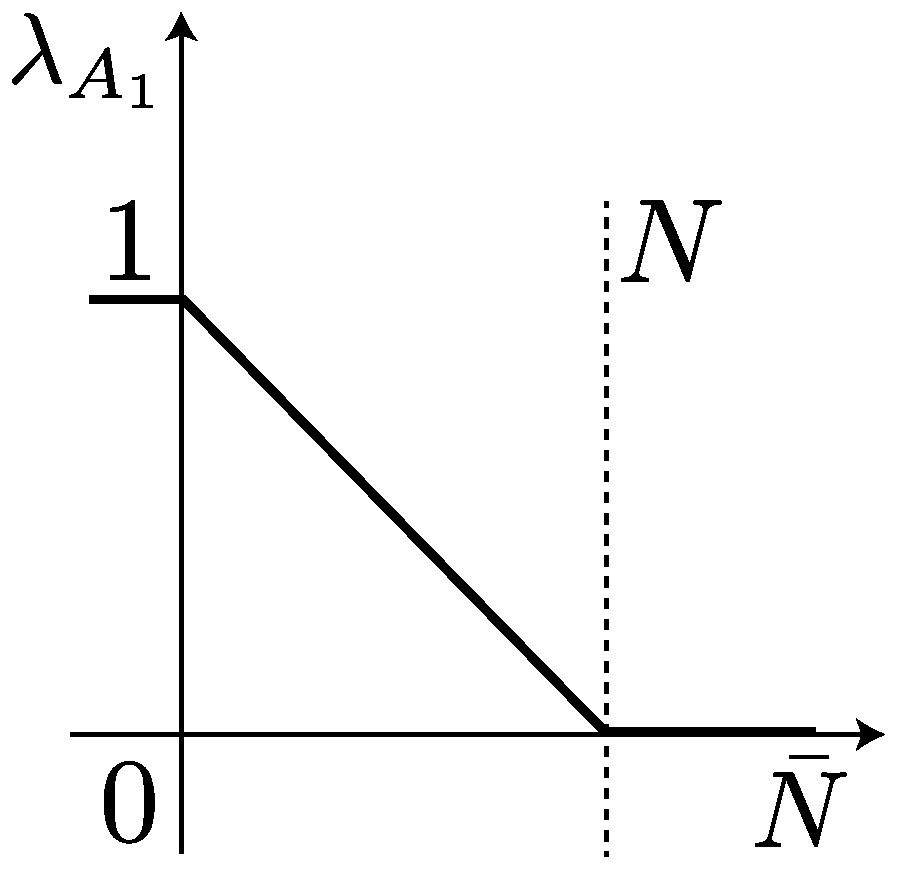
\includegraphics[width=0.40\textwidth]{figure/basic_function_a1}\hfill
	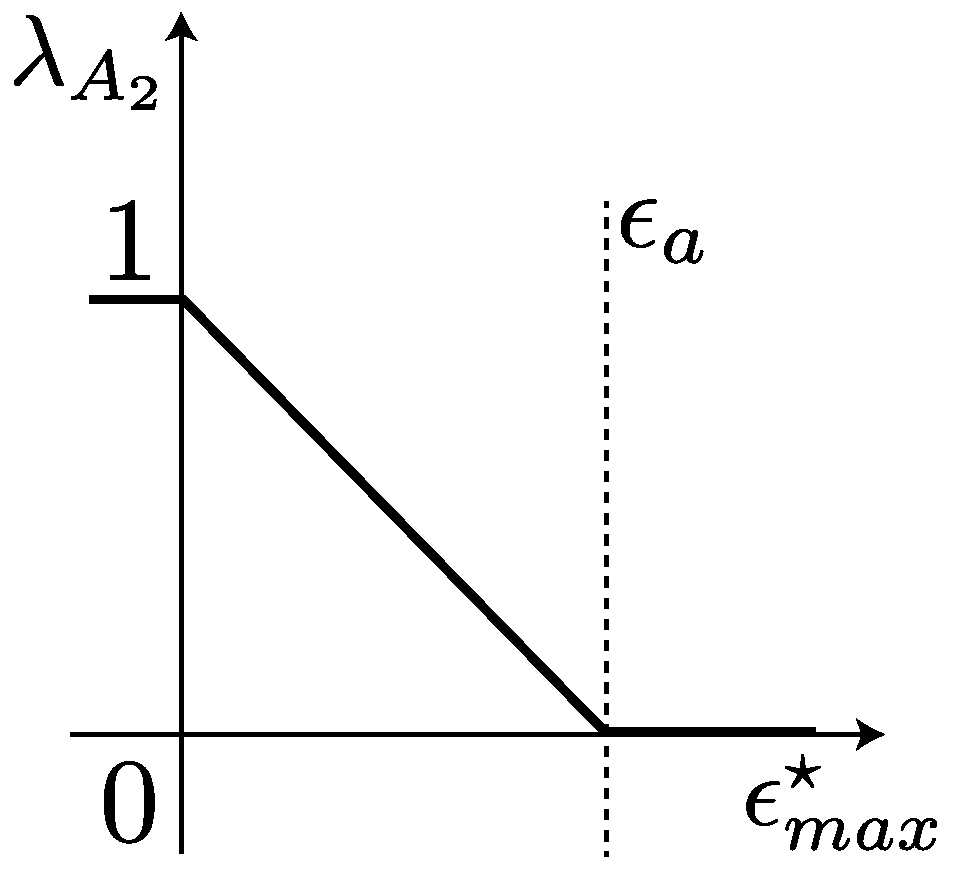
\includegraphics[width=0.43\textwidth]{figure/basic_function_a2}
	\caption{An illustration of the zone-excursion functions defined in \eqref{eq:lambda1} and \eqref{eq:lambda2} for adaptation criteria $(A_1)$ and $(A_2)$, respectively.}\label{fig:zone_functions}%
\end{figure}
\begin{enumerate}[label=(\subscript{A}{{\arabic*}}),leftmargin=40pt]
	\item 	 \textit{settling stage}: given a horizon with $N$ stages, , we select the last stage for which $\epsilon^\star_i \in [\check{\epsilon},\Hat{\epsilon}]$. \textcolor{red}{AF: define this number more formally, assuming that in the last stage the position is within the bounds then it is the minimum $i$ such that the position is in the bounds for $i$ all all the subsequent stages. Otherwise it is just $N$}.
	\textcolor{red}{AF: say that this number represents the 'time' that it would take for the fully automatic controller to bring back the position error within the bound}. 
	This stage is henceforth termed ``active shooting node", $\Bar{N}$ 	\textcolor{red}{AF I would rather call it the 'recovery time' or 'recovery stage'}. The zone-excursion function $\lambda_{A_1} \vcentcolon \mathbb{W} \rightarrow \mathbb{R}$ is defined as:
		\begin{equation}\label{eq:lambda1}%
			\lambda_{A_1} \vcentcolon = \{ \Bar{N} \vcentcolon (N-\Bar{N})/N \in [0,1] \}.
		\end{equation}
	\item \textit{maximum PED in the horizon}: given a horizon with $N$ stages, we select the maximum PED within the horizon, $\epsilon^\star_{max}$, and apply the zone-excursion function $\lambda_{A_2} \vcentcolon \mathbb{R} \rightarrow \mathbb{R}$ characterized as:
		\begin{equation}\label{eq:lambda2}%
			\lambda_{A_2} \vcentcolon = \{\epsilon^\star_{max} \vcentcolon (\epsilon_a-\epsilon^\star_{max})/\epsilon_a \in [0,1] \}.
		\end{equation}
\end{enumerate}

Moreover, assume that $W_R \in \mathbb{R}^{n_{\xi} \times n_{\xi}}, W_H \in \mathbb{R}^{n_{\nu} \times n_{\nu}}$ and $W_C \in \mathbb{R}^{n_u \times n_u}$ are the weight matrices analogous, respectively, to the contribution of the robot, human, and control input in the cost function of $(\mathbf{NLP}_2)$. 
	\textcolor{red}{AF: the control inputs seem not appear in the cost function.}
These matrices contain the initial setting over which the zone-excursion functions modulate the control authority. Thus, we denote the structure of $W(\epsilon_i^\star)$ and ${W}_N(\epsilon_i^\star)$ for both adaptation criteria\footnote{where the underscript $\bullet$ is a wildcard that specifies the zone-excursion function used for building $W(\epsilon_i^\star)$ and ${W}_N(\epsilon_i^\star)$.} as being:

\begin{eqnarray}
\begin{aligned}
	W(\epsilon_i^\star) & =  \text{blkdiag}((1-\lambda_{\bullet})\cdot W_R, \lambda_{\bullet} \cdot W_H, \lambda_{\bullet} \cdot W_C)\\
	{W}_N(\epsilon_i^\star) & = \text{blkdiag}((1-\lambda_{\bullet})\cdot W_R, \lambda_{\bullet} \cdot W_H).\label{eq:weight_matrices}
\end{aligned}
\end{eqnarray}
An illustration of each zone-excursion function is provided in Fig. \ref{fig:zone_functions}.
%%%%%%%%%%%%%%%%%%%%%%%%%%%%%%%%%%%%%%%%%%%%%%%%%%%%%%%%%%%%%%%%%%%%%%%%%%%%%%%%%%%%%%
%%%%%%%%%%%%%%%%%%%%%%%%%%%%%%%%%%%%%%%%%%%%%%%%%%%%%%%%%%%%%%%%%%%%%%%%%%%%%%%%%%%%%%
\section{Numerical Simulations}
In this section, we first provide a detailed description of the navigation task and the implementation. Further we present the simulation results and the computational burden associated with the proposed algorithm.
%%%%%%%%%%%%%%%%%%%%%%%%%%%%%%%%%%%%%%%%%%%%%%%%%%%%%%%%%%%%%%%%%%%%%%%%%%%%%%%%%%%%%%
\subsection{Semi-Autonomous Navigation Task}
The scenario under consideration is inspired by a persistent navigation task in which a person modifies the reference that is autonomously tracked by a robot, rather than piloting the robot itself. The human is assisted by our mixed-initiative control algorithm which allows deformation in the trajectory followed by the robot.

In practice, we would like to use the path calculated by a path planner as reference to $(\mathbf{NLP}_1)$ and the part corresponding to the automatic controller in $(\mathbf{NLP}_2)$. A path is only a sequence of points on the map, typically without heading (orientation of the robot), velocity information, and time indexing. These need to be added before we can use the provided path as reference trajectory in the aforementioned NLPs, which can still be kinodynamically infeasible. When a high-quality reference trajectory (e.g. dynamically feasible, close to a global optimal, etc.) is readily available, it should be used. This can be employed to initialize and thereby drastically speed-up subsequent optimization solutions, and improve the convergence behavior of the algorithm. Nevertheless, a path planner (even a coarse one) is often not available and may be expensive to design or time-consuming to run. Thus, our approach includes a very simple initialization scheme.
%%%%%%%%%%%%%%%%%%%%%%%%%%%%%%%%%%%%%%%%%%%%%%%%%%%%%%%%%%%%%%%%%%%%%%%%%%%%%%%%%%%%%%
\paragraph{Global Reference:} We assume that the time-varying reference in position $p^d$ to be tracked is composed of a simple cartesian helical trajectory, generated using MATLAB. A radius of $r = 0.3$ m is imposed, initial height of $h_0 = 0.35$ m, height increments of $\Delta h = 0.005$ m at each time step, total duration  of $t_f = 6$ s, and $N = 400$ time steps. Moreover, we regulate for $\gamma^d \vcentcolon = (0,0,0)^T$ and $\Omega^d  \vcentcolon = 0.06546\cdot\mathbf{1_4}$, while $v_b^d  \vcentcolon = (0,0,0)^T$ and $\omega^d  \vcentcolon = (0,0,0)^T$.
%%%%%%%%%%%%%%%%%%%%%%%%%%%%%%%%%%%%%%%%%%%%%%%%%%%%%%%%%%%%%%%%%%%%%%%%%%%%%%%%%%%%%%
\paragraph{Human Guidance:} We simulate human actions by means of a reactive controller. Different levels of piloting skills are achieved through three different sets of gain matrices, which significantly improve the tracking performance of the controller. We regard the following control law:
\begin{equation}
\begin{aligned}
	\mathcal{U}_1 &= \mathbf{f}^T_d\mathbf{R}_d\mathbf{1_z}\\
	\mathcal{U}_2 &= - \mathbf{K}_R\mathbf{e}_R - \mathbf{K}_{\omega}\mathbf{e}_{\omega} \end{aligned}\label{eq:control_law}%
\end{equation}
with the respective position, velocity, rotation and angular velocity errors
\begin{equation*}
\begin{aligned}
	\mathbf{e}_p = p - p^d, \quad \mathbf{e}_v = \Dot{p}-\Dot{p}^d, \quad  \mathbf{e}_R = \frac{1}{2}(\mathbf{R}^T_d\mathbf{R}-\mathbf{R}\mathbf{R}_d)^\vee, \quad \mathbf{e}_{\omega} = \omega - \mathbf{R}\mathbf{R}^T_d\omega^d,
\end{aligned}
\end{equation*}
and the following vector
\begin{equation*}
	\mathbf{f}_d = mg\mathbf{1_z} - \mathbf{K}_p\mathbf{e}_p - \mathbf{K}_{v}\mathbf{e}_{v}  -\mathbf{K}_I \int_{t_0}^{t_s}\mathbf{e}_p d\tau,
\end{equation*}
where $\bullet^\vee \vcentcolon SO(3) \rightarrow \mathbb{R}^3$ is the the \emph{vee} operator, and $\mathbf{R} \in SO(3)$ represents the rotation matrix from $\{\mathcal{B}\}$ to $\{\mathcal{I}\}$. The reference attitude trajectory is denoted by $\mathbf{R}_d \in SO(3)$, while $\mathbf{K}_p, \mathbf{K}_v, \mathbf{K}_I, \mathbf{K}_R$ and $\mathbf{K}_{\omega}$ are positive definite gain matrices.

The control law in \eqref{eq:control_law} provides the nominal input required to track the full-pose trajectory $q = (p^d, R_d) \vcentcolon [t_0,t_f]\rightarrow SE(3)$, retrieved from the global reference. The matrix $\mathbf{R}_d$ and the nominal input can be transformed into desired attitude and speed of the propellers (see Appendix \ref{ap:human_commands}), which are passed to (\textbf {NLP$_2$}) as a reference trajectory. In this way, as long as the adaptive criterion is met, the human inputs will retain the control authority and modify the reference tracked by the robot.

The levels of piloting skills considered are inexperienced (\textbf{L0}), intermediate (\textbf{L1}) and experienced (\textbf{L2}).
%%%%%%%%%%%%%%%%%%%%%%%%%%%%%%%%%%%%%%%%%%%%%%%%%%%%%%%%%%%%%%%%%%%%%%%%%%%%%%%%%%%%%%
%%%%%%%%%%%%%%%%%%%%%%%%%%%%%%%%%%%%%%%%%%%%%%%%%%%%%%%%%%%%%%%%%%%%%%%%%%%%%%%%%%%%%%
\subsection{Implementation Details}
\paragraph{Nonlinear Optimization via Real-Time Iteration Scheme:} In real-time NMPC applications, (\textbf{NLP$_1$}) and (\textbf{NLP$_2$}) need to be solved at each sampling instant under the available computation time. To that end, we use a numerical strategy based on \emph{sequential quadratic programming} (SQP) that relies on the solution of a limited number of quadratic program (QP) subproblems, the so-called real-time iteration (RTI) scheme. More precisely, in this strategy only a single linearization and QP solve are carried out per sampling instant, leading to an approximate feedback control policy. An important ingredient in the RTI scheme is to keep the initial state as a constrained decision variable, which is often referred to as \emph{initial value embedding}. This allows one to divide computations into a preparation and a feedback phase, where the former is typically more expensive. In this work, we will be using the implementation of the RTI method by means of the high-performance software package \texttt{acados}.

The \emph{direct multiple shooting} approach is used in order to obtain (\textbf{NLP$_1$}) and (\textbf{NLP$_2$}). The state trajectories from stage 0 to $N$ are approximated using a numerical integration scheme, in this case an explicit Runge Kutta 4th order (ERK4), while the input trajectories are parametrized as piecewise constant. We make use of \texttt{acados} Python template-based interface to generate the libraries that implement (\textbf{NLP$_1$}) and (\textbf{NLP$_2$}), which are then wrapped by our mixed-initiative control algorithm, written in Python, which executes Algorithm 1. 

\IncMargin{1em}
\begin{algorithm}
\SetKwInOut{Input}{Input}\SetKwInOut{Output}{Output}
\Input{States $\Bar{\xi}_{0(k)},\Bar{\sigma}_{0(k)}$ and references $\Bar{\eta}_{(k)},\Tilde{\eta}_{(k)}$ at iteration $k$.}
\Output{Solution $(\sigma_i,u_i)_k$ for (\textbf{NLP$_2$}$)_k$ at iteration $k$.}
\KwData{maximum admissible error $a = (0.05,0.05,0.1)$ m, \textit{criterion}, simulation time $t_f$ = 6 s, sampling time $t_s = 0.015$ s.}
\BlankLine
\Begin{
	$k \longleftarrow 0$\;
	Calculate $\epsilon_a$ in \eqref{eq:aed}\;
	$\check{\epsilon} \longleftarrow 0$\;
	$\Hat{\epsilon} \longleftarrow \epsilon_a$\;
	\For{$k \longleftarrow 0$ \KwTo $t_f/t_s$}{
		Update $\Bar{\eta}_{(k)}$\;
		Solve (\textbf{NLP$_1$}$)_k$ for $\Bar{\xi}_{0(k)}$\;
		\For{$i \longleftarrow 0$ \KwTo $N$}{
			Calculate $\epsilon^\star_{i(k)}$ in \eqref{eq:ped}\;
		}
		\If{criterion = $(A_1)$}{
			\For{$i \longleftarrow N$ \KwTo $0$}{
				\If{$\epsilon^\star_{i(k)} < \Hat{\epsilon}$}{
      				$\Bar{N}_{i(k)} \longleftarrow \texttt{NaN}$\;
    			}
    			\Else{$\Bar{N}_{i(k)} \longleftarrow i$\;}{	
    			}
    		}
    		$\Bar{N}_{(k)} \longleftarrow$ last non-\texttt{NaN} element of $\Bar{N}_{i(k)}$\;
    		Evaluate zone-excursion function $\lambda_{A_1(k)}$ in \eqref{eq:lambda1}\;
    	}
    	\If{criterion = $(A_2)$}{
			\For{$i \longleftarrow N$ \KwTo $0$}{
				\If{$\epsilon^\star_{i(k)} > \Hat{\epsilon}$}{
      				$\epsilon^\star_{i(k)} \longleftarrow \Hat{\epsilon}$\;
    			}
    			$\epsilon^\star_{i,max(k)} \longleftarrow \epsilon^\star_{i(k)}$\;
    			
			}
			$\epsilon^\star_{max(k)} \longleftarrow \text{max}(\epsilon^\star_{i,max(k)})$\;
			Evaluate zone-excursion function $\lambda_{A_2(k)}$ in \eqref{eq:lambda2}\;
		}
		Build $W(\epsilon^\star_{i(k)})$ and ${W}_N(\epsilon^\star_{i(k)})$ in \eqref{eq:weight_matrices}\;
		Calculate $\mathcal{U}_{1(k)}$ and $\mathcal{U}_{2(k)}$ in \eqref{eq:control_law}\; 
		Simulate human commands based on $\mathbf{R}_{d(k)}$, $\mathcal{U}_{1(k)}$ and $\mathcal{U}_{2(k)}$\;
		Update $\Tilde{\eta}_{(k)}$\;
		Solve (\textbf{NLP$_2$}$)_k$ for $\Bar{\sigma}_{0(k)}$\;
		\Return $(\sigma_i, u_i)_k$
	}
}
\caption{zone NMPC for mixed-initiative control}\label{algo:zonenmpc}
\end{algorithm}\DecMargin{1em}
%%%%%%%%%%%%%%%%%%%%%%%%%%%%%%%%%%%%%%%%%%%%%%%%%%%%%%%%%%%%%%%%%%%%%%%%%%%%%%%%%%%%%%
\paragraph{Structure-exploiting QP Solver and Condensing Approach:} The QPs arising in both NMPC formulations are addressed using the high-performance interior-point method (\texttt{HPIPM}) solver that is built on top of the linear algebra package \texttt{BLASFEO}. This Riccati-based solver implements an efficient method for the solution of linear-quadratic (LQ) control problem, that is a special instance of equality constrained quadratic program. The corresponding Karush-Kuhn-Tucker (KKT) system is sparse and structured, and this structure is exploited by \texttt{HPIPM} which grants a reduction in the number of flops. As for the linear algebra library, the major difference between existing high-performance implementations of BLAS-- and LAPACK--like routines for embedded applications and \texttt{BLASFEO} is that the last is optimized for small to medium scale matrices. The \texttt{X64\_INTEL\_HASWELL} implementation of \texttt{BLASFEO} package was used, which exploits a set of vectorized instructions for the target CPU. 

Additionally, for the NMPC solutions, we used partial condensing \texttt{HPIPM}-based technique. 
This approach reformulates the large and sparse Hessians of (\textbf{NLP$_1$}) and (\textbf{NLP$_2$}) into small and dense ones, which have a more suitable form for the QP solver. 
%%%%%%%%%%%%%%%%%%%%%%%%%%%%%%%%%%%%%%%%%%%%%%%%%%%%%%%%%%%%%%%%%%%%%%%%%%%%%%%%%%%%%%
\paragraph{Parametrization of Mixed-Initiative Control Algorithm:} To what concerns the parametrization of both NLPs, we assume a sampling time of $t_s = 15$ ms, and $N=50$ shooting nodes. The values of the parameters appearing in the model are listed in Table \ref{tab:prm}. Constraints for this system include bounds on speed $\ubar{\Omega} = 0$, $\Bar{\Omega} = 0.09$ kHz, and control $\ubar{u} = 0$, $\Bar{u} =  0.1285$ kNm. The weight matrices of the low-level NMPC are
\begin{equation*}
\begin{aligned}
	W & = \text{blkdiag}(250\cdot\mathbf{I_2},300, 30\cdot\mathbf{I_3},5\cdot\mathbf{I_6},30\cdot\mathbf{I_4},70\cdot\mathbf{I_4}), \\
	W_N & = \text{blkdiag}(250\cdot\mathbf{I_2},300, 30\cdot\mathbf{I_3},5\cdot\mathbf{I_6},30\cdot\mathbf{I_4}).
\end{aligned}
\end{equation*}
Similarly, the weight matrices for the initial setting of the zone NMPC are
\begin{equation*}
\begin{aligned}
		W_R & = \text{blkdiag}(250\cdot\mathbf{I_2},300, 30\cdot\mathbf{I_3},5\cdot\mathbf{I_6},30\cdot\mathbf{I_4}),\\
		W_H & = \text{blkdiag}(30\cdot\mathbf{I_3},5\cdot\mathbf{I_3},30\cdot\mathbf{I_4}),\\
		W_C & = 70\cdot\mathbf{I_4}.
\end{aligned}
\end{equation*}
Notice that the weights assigned to the human contribution have the same values as their corresponding part in the robot contribution (i.e. Euler angles, angular rates and speed of the propellers). This is done in order to preserve equality of modulation-range.  

Finally, the maximum deformation conceded to the human with respect to the reference of the robot is $a \vcentcolon = (0.05,0.05,0.1)$ m, causing the bounds on the target zone to be $\check{\epsilon}=0, \Hat{\epsilon} = 0.122$ m.

\begin{table}[h]
\caption{Quadrotor model - values of the parameter used for the simulation results in this section.}\label{tab:prm}
\begin{tabular}{ccc}
\hline
\textbf{Parameter} & \textbf{Value}                                  & \textbf{Description}                               \\ \hline
$g$       & 9.8066 m/s$^2$                         & gravitational acceleration                \\ \hline
$m$       & 1.04 kg                                & total mass                                \\ \hline
$l$       & 0.23 m                               & arm length    \\ \hline
$J_{xx}$    & $0.010$ kg $\cdot$ m$^2$ & inertia moment around x \\ \hline
$J_{yy}$    & $0.010$ kg $\cdot$ m$^2$ & inertia moment around y \\ \hline
$J_{zz}$    & $0.070$ kg $\cdot$ m$^2$ & inertia moment around z \\ \hline
$C_D$     & $10.0$ Nm/kHz     & drag coefficient                          \\ \hline
$C_T$     & $595.0$ N/kHz        & thrust coefficient                        \\ \hline
$J_m$	  & $0.8$ kg $\cdot$ m$^2$ & rotor inertia \\ \hline
\end{tabular}
\end{table}
%%%%%%%%%%%%%%%%%%%%%%%%%%%%%%%%%%%%%%%%%%%%%%%%%%%%%%%%%%%%%%%%%%%%%%%%%%%%%%%%%%%%%%
%%%%%%%%%%%%%%%%%%%%%%%%%%%%%%%%%%%%%%%%%%%%%%%%%%%%%%%%%%%%%%%%%%%%%%%%%%%%%%%%%%%%%%
\newpage
\subsection{Performance Analysis}
In the simulations we assess the effectiveness of the mixed-initiative control algorithm in terms of whether or not human operators are afforded the freedom that is required to modify the reference tracked by the robot, regardless of the level of piloting skill. Additionally, we would like to measure the performance of the navigation task for the two adaptation criteria presented. Figure \ref{fig:l0_a1}--\ref{fig:l2_a2} show the results for six different simulations in which Algorithm 1 was used. Independently of the criterion used to compute $\lambda_{\bullet}$, the values $\lambda_{\bullet} = 0.0, \lambda_{\bullet} \in \mathbb{R} = (0.0,1.0), \lambda_{\bullet} = 1.0$ indicate \emph{fully automatic control}, \emph{shared control} and \emph{fully human control}, respectively.

The graphs depict the evolution of both zone-excursion functions $\lambda_{\bullet}$ for which the insets show the corresponding unfolding of either $\Bar{N}$ or $\epsilon^\star_{max}$. It is also shown the predicted Euclidean distances $\epsilon^\star_i$ analogous to the time interval of the inset. The light blue and pink colors in the graphs for criterion $(A_1)$ indicate the predicted Euclidian distances that are within and exceed the target zone, respectively, e.g. $\Bar{N} = 0$ and $\Bar{N} \in \mathbb{W} = [1,50]$. In contrast, for criterion $(A_2)$ pink corresponds to $\epsilon^\star_{max} \in \mathbb{R} = (0.0,1.0)$.

When $\Bar{N} \in \mathbb{W} = [1,50]$, i.e. PED exceeds the target zone, then $0 <\lambda_{A_1} \leq 1$, resulting in a reduction in the human control authority while $\lim_{\Bar{N}\to 50}\lambda_{A_1}(\Bar{N})$, according to \eqref{eq:weight_matrices}. In general, the insets of $\lambda_{A_1}$ show that, when active, the zone NMPC starts producing a precipitous fall in the human control authority. However, due to the high level of ``trust in the human" embedded in criterion $(A_1)$, this off-peak is short-lived. Because of the settling stage-weighting, the active shooting node is gradually decreased, with respect to previous NMPC solutions, right after the main $\lambda_{A_1}$ off-peak. This decrease corresponds to the transition from the shared control phase, in which $\epsilon^\star_i$ exceeds the target zone, to the phase fully controlled by the human, in which $\epsilon^\star_i$ undulates nonchalantly within $[\check{\epsilon},\Hat{\epsilon}]$, accruing no extra penalization, as $\Bar{N}$ remains equal to zero. 

On the other hand, when using criterion $(A_2)$, the zone NMPC persistently opts for stark shared control throughout the task. The aim of zone-excursion function $\lambda_{A_2}$ is to aggressively reduce human control authority only an increasing in the error margin arises, indicating that this is a criterion with a low level of ``trust in the human". Maximum PED-weighting constantly attenuates human control authority compared with using the fixed nominal weights and, for this reason, is inherently safer as it is ``active" at each prediction step.

The simulation results have shown that the proposed mixed-initiative control algorithm is able to provide to the human operator the freedom to modify the reference tracked by the robot, no matter the level of piloting skill. Proposed zone NMPC with criterion $(A_1)$ yields an oscillatory, albeit slightly more sluggish, return to the target zone. Instead, proposed zone NMPC with criterion $(A_2)$ does not exceed the target zone whatsoever. As maximum PED-weighting ends up being continuously ``active", it is advantageous for more challenging situations, for instance, with an inexperienced pilot, capable of reducing the human workload and also providing higher performance benefits.

%%%%%%%%%%%%%%%%%%%%%%%%%%%%%%%%%%%%%%%%%%%%%%%%%%%%%%%%%%%%%%%%%%%%%%%%%%%%%%%%%%%%%%
%%%%%%%%%%%%%%%%%%%%%%%%%%%%%%%%%%%%%%%%%%%%%%%%%%%%%%%%%%%%%%%%%%%%%%%%%%%%%%%%%%%%%%
\newpage
\paragraph{Inexperienced $(\mathbf{L0})$:} Closed-loop results for mixed-initiative control algorithm.
\begin{figure*}[h]\centering
	\includegraphics[width=1.0\textwidth]{../../Software/plots/case0/noob/position}
	\caption{Using adaptation criterion ($A_1$).}\label{fig:l0_a1}%
	\vspace{0.5cm}
	\includegraphics[width=1.0\textwidth]{../../Software/plots/case1/noob/position}
	\caption{Using adaptation criterion ($A_2$).}\label{fig:l0_a2}%
\end{figure*}
%%%%%%%%%%%%%%%%%%%%%%%%%%%%%%%%%%%%%%%%%%%%%%%%%%%%%%%%%%%%%%%%%%%%%%%%%%%%%%%%%%%%%%
\newpage
\paragraph{Intermediate $(\mathbf{L1})$:} Closed-loop results for mixed-initiative control algorithm.
\begin{figure*}[h]\centering
	\includegraphics[width=1.0\textwidth]{../../Software/plots/case0/inter/position}
	\caption{Using adaptation criterion ($A_1$).}\label{fig:l1_a1}%
	\vspace{0.5cm}
	\includegraphics[width=1.0\textwidth]{../../Software/plots/case1/inter/position}
	\caption{Using adaptation criterion ($A_2$).}\label{fig:l1_a2}%
\end{figure*}
%%%%%%%%%%%%%%%%%%%%%%%%%%%%%%%%%%%%%%%%%%%%%%%%%%%%%%%%%%%%%%%%%%%%%%%%%%%%%%%%%%%%%%
\newpage
\paragraph{Experienced $(\mathbf{L2})$:} Closed-loop results for mixed-initiative control algorithm.
\begin{figure*}[h]\centering
	\includegraphics[width=1.0\textwidth]{../../Software/plots/case0/pro/position}
	\caption{Using adaptation criterion ($A_1$).}\label{fig:l2_a1}%
	\vspace{0.5cm}
	\includegraphics[width=1.0\textwidth]{../../Software/plots/case1/pro/position}
	\caption{Using adaptation criterion ($A_2$).}\label{fig:l2_a2}%
\end{figure*}
%%%%%%%%%%%%%%%%%%%%%%%%%%%%%%%%%%%%%%%%%%%%%%%%%%%%%%%%%%%%%%%%%%%%%%%%%%%%%%%%%%%%%%
%%%%%%%%%%%%%%%%%%%%%%%%%%%%%%%%%%%%%%%%%%%%%%%%%%%%%%%%%%%%%%%%%%%%%%%%%%%%%%%%%%%%%%
%%%%%%%%%%%%%%%%%%%%%%%%%%%%%%%%%%%%%%%%%%%%%%%%%%%%%%%%%%%%%%%%%%%%%%%%%%%%%%%%%%%%%%
\newpage
\subsection{Computational Burden}
Computation times reported are from an Intel Core i5 $@2.6$ GHz running macOS Catalina. Whether the sparse, condensed or partially condensed formulation is more appropriate for a certain problem depends mainly on the horizon length and the ratio between number of states and controls. In this particular problem, we note that the partially condensed QP is more beneficial from a computational point of view. \texttt{HPIPM} is significantly faster in solving the partially condensed QP arising in each NMPC formulation compared to the corresponding dense QP (see Table \ref{tab:cputime_pc} and \ref{tab:cputime_c}). The dense solver \texttt{qpOASES} was also tested, but did not return a solution for any of the attempts.

In the condensed formulation, all state deviations are eliminated via the continuity constraints of (\textbf{NLP$_1$}) and (\textbf{NLP$_2$}) leading to a smaller but dense QP. Conversely, partial condensing is a condensing strategy that is in-between the sparse and the fully condensed formulations. In this strategy, a state component is retained as an optimization variable at each stage of the partially condensed QP. Given the dimensions of the optimal control problems (OCP) involved in our mixed-initiative control algorithm, partial condensing allows to better exploit hardware throughput.

\begin{table}[h]
\caption{Average computation times in [ms] for partial condensing.}
\begin{tabular}{lccccccc}
\toprule
\multirow{2}[3]{*}{} & & \multicolumn{2}{c}{} & \multicolumn{2}{c}{\texttt{HPIPM}}\\
\cmidrule(lr){3-8}
 & \multirow{2}[3]{*}{Condensing approach} & \multicolumn{2}{c}{\textbf{L0}} & \multicolumn{2}{c}{\textbf{L1}} & \multicolumn{2}{c}{\textbf{L2}}\\
\cmidrule(lr){3-4} \cmidrule(lr){5-6} \cmidrule(lr){7-8}
 & & $(A_1)$ & $(A_2)$ & $(A_1)$ & $(A_2)$ & $(A_1)$ & $(A_2)$\\
\midrule
LL NMPC\footnotemark & \textit{partial condensing} & 4.92 & 4.51 & 4.53 & 4.04 & 4.05 & 3.88 \\
\midrule
zone NMPC & \textit{partial condensing} & 10.09 & 9.74 & 7.58 & 7.62 & 6.83 & 7.51 \\
\bottomrule
\end{tabular}\label{tab:cputime_pc}
\end{table}

\begin{table}[h]
\caption{Average computation times in [ms] for condensing.}
\begin{tabular}{lccccccc}
\toprule
\multirow{2}[3]{*}{} & & \multicolumn{2}{c}{} & \multicolumn{2}{c}{\texttt{HPIPM}}\\
\cmidrule(lr){3-8}
 & \multirow{2}[3]{*}{Condensing approach} & \multicolumn{2}{c}{\textbf{L0}} & \multicolumn{2}{c}{\textbf{L1}} & \multicolumn{2}{c}{\textbf{L2}}\\
\cmidrule(lr){3-4} \cmidrule(lr){5-6} \cmidrule(lr){7-8}
 & & $(A_1)$ & $(A_2)$ & $(A_1)$ & $(A_2)$ & $(A_1)$ & $(A_2)$\\
\midrule
LL NMPC & \textit{condensing} & 9.67 & 8.43 & 8.53 & 7.30 & 7.78 & 7.15 \\
\midrule
zone NMPC & \textit{condensing} & 14.07 & 13.60 & 10.47 & 10.74 & 9.43 & 10.08 \\
\bottomrule
\end{tabular}\label{tab:cputime_c}
\end{table}

\footnotetext{shorthand for low-level NMPC.}
%%%%%%%%%%%%%%%%%%%%%%%%%%%%%%%%%%%%%%%%%%%%%%%%%%%%%%%%%%%%%%%%%%%%%%%%%%%%%%%%%%%%%%
%%%%%%%%%%%%%%%%%%%%%%%%%%%%%%%%%%%%%%%%%%%%%%%%%%%%%%%%%%%%%%%%%%%%%%%%%%%%%%%%%%%%%%
\begin{appendix}
\chapter{Appendix}
\section{Generation of Human Commands}\label{ap:human_commands}
Given the reference attitude $\mathbf{R}_d$ and the nominal input $(\mathcal{U}_1,\mathcal{U}_2)$, it is possible to determine the desired attitude ($\phi^d_h,\theta^d_h, \psi^d_h$) and speed of the propellers ($\Omega^d_{h,[1,4]}$) that correspond to the human inputs. We will define the following parametrization of the rotation matrix:
\begin{equation*}
	\mathbf{R}_d = \begin{pmatrix} cos\theta cos\psi & -cos\phi sin\psi + sin\phi sin\theta cos\psi & sin\phi sin\psi + cos\phi cos\theta cos\psi \\
	cos\theta sin\psi & cos\phi sin\psi + sin\phi sin\theta sin\psi & -sin\theta cos\psi + cos\phi sin\theta sin\psi \\
	-sin\theta & sin\phi cos\theta & cos\phi cos\theta	
	\end{pmatrix}.
\end{equation*}

Based on that, one can compute the desired attitude by doing:
\begin{equation*}
\begin{aligned}
	\phi^d_h = \text{atan2}\left( \frac{\mathbf{R}_{d,32}}{\mathbf{R}_{d,33}} \right), \quad \theta^d_h = -\text{asin}\left ( \mathbf{R}_{d,31} \right ), \quad \psi^d_h = \text{atan2}\left( \frac{\mathbf{R}_{d,21}}{\mathbf{R}_{d,11}} \right).
\end{aligned}
\end{equation*}

Moreover, to compute the desired speed of the propellers we assume control decoupling. First, we linearize the forces and moments in \eqref{eq:force_moments} and rewrite them in the following matrix format:
\begin{equation}
	\begin{pmatrix}F_z \\M_x \\M_y \\M_z \end{pmatrix} = 2\Omega_e\underbrace{\begin{pmatrix} C_T & C_T & C_T & C_T \\
	-C_Tl & -C_Tl & C_Tl & C_Tl \\
	-C_Tl & C_Tl & C_Tl & -C_Tl \\
	-C_D & C_D & -C_D & C_D
	\end{pmatrix}}_{\mathbf{\Gamma}}
	\begin{pmatrix}\Delta \Omega_1\\ \Delta \Omega_2\\ \Delta \Omega_3\\ \Delta \Omega_4\end{pmatrix},\label{eq:gamma}%
\end{equation}
where $\Omega_e$ is the required speed of each rotor in order to maintain the hover position, and the prefix $\Delta$ indicates the result of a linearization process.

Second, if matrix $\mathbf{\Gamma}$ is invertible, then the lines are linearly independent, meaning that the forces and moments acting on the CoM of the quadrotor are independently from each other. The inverse relation  of \eqref{eq:gamma} is given by
\begin{equation}
\begin{pmatrix}\Delta \Omega_1\\ \Delta \Omega_2\\ \Delta \Omega_3\\ \Delta \Omega_4\end{pmatrix} = \frac{1}{2\Omega_e}\underbrace{\begin{pmatrix}
1/(4C_T) & -1/(4C_Tl) & -1/(4C_Tl) & -1/(4C_D)\\
1/(4C_T) & -1/(4C_Tl) & 1/(4C_Tl) & 1/(4C_D)\\
1/(4C_T) & 1/(4C_Tl) & 1/(4C_Tl) & -1/(4C_D)\\
1/(4C_T) & 1/(4C_Tl) & -1/(4C_Tl) & 1/(4C_D)
\end{pmatrix}}_{\mathbf{\Gamma}^{-1}}
\begin{pmatrix}F_z \\M_x \\M_y \\M_z \end{pmatrix}.\label{eq:gamma_inv}%
\end{equation}

The inverse mapping \eqref{eq:gamma_inv} dictates how each of the forces acting on the CoM of the quadrotor contributes to the rotation speed of each propeller. We can use this fact to establish the relation between the nominal input of the reactive controller and the desired speed of the propellers, which are further passed on to (\textbf{NLP}$_2$). Consequently, we have that
\begin{equation*}
\begin{pmatrix}\Omega^d_{h,1}\\ \Omega^d_{h,2}\\ \Omega^d_{h,3}\\ \Omega^d_{h,4}\end{pmatrix} = \frac{1}{2\Omega_e}\mathbf{\Gamma}^{-1}\begin{pmatrix}\mathcal{U}_{1,z}\\ \mathcal{U}_2\end{pmatrix},
\end{equation*}
where $\mathcal{U}_{1,z}$ is the $z$ component of vector $\mathcal{U}_1$.
\end{appendix}



\end{document}
